\newpage
\section{Integration (multi-variat)}
% TODO: Koordinatentransformation (Längenverzerrung, Elementverzerrung, Längenelement)
\subsection{Dreidimensionale Koordinatensysteme}
\resizebox{\linewidth}{!}{
    \begin{tabular}{c c c}
        \myul{\textbf{Kartesisch}} & \myul{\textbf{Zylindrisch}} & \myul{\textbf{Kubisch}} \\
        
        \tdplotsetmaincoords{70}{110}
        \begin{tikzpicture}[tdplot_main_coords, scale=2]
            % Koordinatensystem
            \draw [->] (0, 0, 0) -- (1, 0, 0) node [below left] {$x$};
            \draw [->] (0, 0, 0) -- (0, 1, 0) node [right]      {$y$};
            \draw [->] (0, 0, 0) -- (0, 0, 1) node [right]      {$z$};
            % Punkt bei (0.75,0.75,0.75)
            \fill (0.75, 0.75, 0.75) circle (1pt) node [above right] {$P(x, y, z)$};
            % Koordinatenkomponenten
            \draw [dashed] (0, 0.75, 0)    -- (0.75, 0.75, 0)    node [midway, below right] {$x$};
            \draw [dashed] (0.75, 0, 0)    -- (0.75, 0.75, 0)    node [midway, below left]  {$y$};
            \draw [dashed] (0.75, 0.75, 0) -- (0.75, 0.75, 0.75) node [midway, right]       {$z$};
        \end{tikzpicture} &

        \tdplotsetmaincoords{70}{110}
        \begin{tikzpicture}[tdplot_main_coords, scale=2]
            % Koordinatensystem
            \draw [->] (0, 0, 0) -- (1, 0, 0) node [below left] {$x$};
            \draw [->] (0, 0, 0) -- (0, 1, 0) node [right]      {$y$};
            \draw [->] (0, 0, 0) -- (0, 0, 1) node [right]      {$z$};
            % Punkt bei (0.75,0.75,0.75)
            \fill (0.75, 0.75, 0.75) circle (1pt) node [above right] {$P(r, \phi, z)$};
            % Koordinatenkomponenten
            \draw [dashed] (0,0,0)         --  (0.75, 0.75, 0)    node [midway, above right] {$r$};
            \draw [->]     (0.5,0,0)       arc (0:45:0.5)         node [midway, below]       {$\phi$};
            \draw [dashed] (0.75, 0.75, 0) --  (0.75, 0.75, 0.75) node [midway, right]       {$z$};
        \end{tikzpicture} &

        \tdplotsetmaincoords{70}{110}
        \begin{tikzpicture}[tdplot_main_coords, scale=2]
            % Koordinatensystem
            \draw [->] (0, 0, 0) -- (1, 0, 0) node [below left] {$x$};
            \draw [->] (0, 0, 0) -- (0, 1, 0) node [right]      {$y$};
            \draw [->] (0, 0, 0) -- (0, 0, 1) node [right]      {$z$};
            % Punkt bei (0.75,0.75,0.75)
            \fill (0.75, 0.75, 0.75) circle (1pt) node [above right] {$P(r, \theta, \phi)$};
            % Koordinatenkomponenten
            \draw [dotted] (0,0,0) -- (0.75, 0.75, 0) -- (0.75, 0.75, 0.75);
            \draw [->]     (0.5,0,0) arc (0:45:0.5)         node [midway, below]       {$\phi$};
            \draw [dashed] (0, 0, 0) --  (0.75, 0.75, 0.75) node [midway, below right] {$r$};
            \tdplotsetthetaplanecoords {90}
            \tdplotdrawarc [tdplot_rotated_coords, ->] {(0, 0, 0)} {0.5} {0} {45} {anchor=south} {$\theta$}
        \end{tikzpicture} \\

        $ 
        \begin{pmatrix}
            x \\ y \\ z
        \end{pmatrix} 
        =
        \begin{pmatrix}
            r \cos \phi \\ r \sin \phi \\ z
        \end{pmatrix}
        =
        \begin{pmatrix}
            r \sin \theta \cos \phi \\ r \sin \theta \sin \phi \\ r \cos \theta
        \end{pmatrix}
        $ &
        $ 
        \begin{pmatrix}
            r_{zyl} \\ \phi \\ z
        \end{pmatrix} 
        =
        \begin{pmatrix}
            \sqrt{x^2 + y^2} \\ \tan^{-1}\frac{y}{x} \\ z
        \end{pmatrix}
        =
        \begin{pmatrix}
            r_{sph} \sin \theta \\ \phi \\ r_{sph} \cos \theta
        \end{pmatrix}
        $ &
        $ 
        \begin{pmatrix}
            r_{sph} \\ \theta \\ \phi
        \end{pmatrix} 
        =
        \begin{pmatrix}
            \sqrt{x^2+y^2+z^2} \\ \cos^{-1} \frac{z}{r_{sph}} \\ \sgn(y) \cos^{-1} \frac{x}{\sqrt{x^2+y^2}}
        \end{pmatrix}
        =
        \begin{pmatrix}
            \sqrt{r_{zyl}^2+z^2} \\ \tan^{-1}\frac{r_{zyl}}{z} \\ \phi
        \end{pmatrix}
        $ \\
    \end{tabular}
}
\smallskip
\subsubsection{Umrechnen zwischen Koordinatensystemen}
Beim Umrechnen zwischen den Koordinatensystemen gelten im Grunde genommen die obigen Formeln. 
Dabei muss jedoch in einigen Fällen auf die Wertebereiche von den trigonometrischen Funktionen rücksicht genommen werden.

\myul{\textbf{Zylindrisch $\rightarrow$ Kartesisch:}}\\
\myul{\textbf{Sphärisch $\rightarrow$ Kartesisch:}}\\
Keine weiteren Berücksichtigungen nötig, die Berechnung erfolgt nach der Formel oben.
\medskip

\myul{\textbf{Kartesisch $\rightarrow$ Zylindrisch:}}\\
\begin{minipage}{0.49\linewidth}
    Der Parameter $\phi$ wird analog zum zweidimensionalen Fall, je nach dem in welchem Quadranten sich $P$ befindet, nach dem Schema rechts berechnet.
\end{minipage}
\hfill
\begin{minipage}{0.49\linewidth}
    \begin{center}
        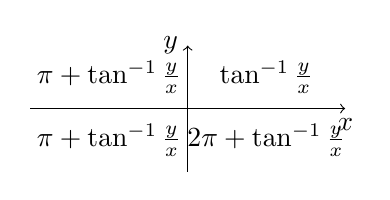
\begin{tikzpicture}
            % Achsen 
            \draw [->] (-2, 0) -- (2, 0) node [below] {$x$};
            \draw [->] (0, -0.8) -- (0, 0.8) node [left] {$y$};
            % Formeln
            \node at ( 1,  0.4) {$       \tan^{-1}\frac{y}{x}$};
            \node at ( 1, -0.4) {$2\pi + \tan^{-1}\frac{y}{x}$};
            \node at (-1, -0.4) {$ \pi + \tan^{-1}\frac{y}{x}$};
            \node at (-1,  0.4) {$ \pi + \tan^{-1}\frac{y}{x}$};
        \end{tikzpicture}
    \end{center}
\end{minipage}
\medskip

\myul{\textbf{Sphärisch $\rightarrow$ Zylindrisch:}}\\
\myul{\textbf{Kartesisch $\rightarrow$ Sphärisch:}}\\
Keine weiteren Berücksichtigungen nötig, die Berechnung erfolgt nach der Formel oben.
\medskip

\myul{\textbf{Zylindrisch $\rightarrow$ Sphärisch:}}\\
\begin{minipage}{0.49\linewidth}
    Auch hier macht der $\tan^{-1}$ Probleme, da er Werte von $-\frac{\pi}{2}$ bis $\frac{\pi}{2}$ liefert, für $\theta$ jedoch $\theta \in [0, \pi]$ gelten soll.
    Je nach dem, ob $P$ sich oberhalb oder unterhalb der $xy$-Ebene befindet, wird $\theta$ wie rechts berechnet.
\end{minipage}
\hfill
\begin{minipage}{0.49\linewidth}
    \begin{center}
        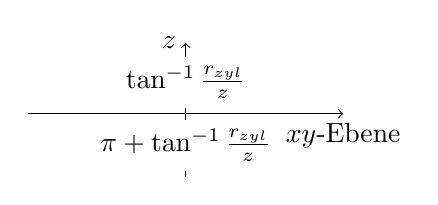
\begin{tikzpicture}
            % Achsen 
            \draw [->] (-2,  0)   -- (2, 0) node [below] {$xy$-Ebene};
            \draw [->] ( 0, -0.8) -- (0,.9) node [left]  {$z$};
            % Formeln
            \node [fill=white] at (0,  0.4) {$\tan^{-1}\frac{r_{zyl}}{z}$};
            \node [fill=white] at (0, -0.4) {$\pi + \tan^{-1}\frac{r_{zyl}}{z}$};
        \end{tikzpicture}
    \end{center}
\end{minipage}

\subsection{Längenintegrale}
\subsubsection{Längenelemente}\label{section:int_multivar:längenelemente}
$$
 \diff s^2 
    = \underbrace{\diff x^2 + \diff y^2 + \diff z^2}_{\text{Kartesisch}}
    = \underbrace{\diff r^2 + r^2 \diff \theta^2 + \diff z^2}_{\text{Zylindrisch}}
    = \underbrace{\diff r^2 + r^2 \diff \theta^2 + r^2 \sin^2 \theta \diff \phi^2}_{\text{Sphärisch}}
$$
\subsubsection{Länge einer Funktion}
Die Bestimmung der Länge einer Kurve kann in folgende Schritte unterteilt werden:
\begin{enumerate}
    \item \myul{\textbf{Funktion in die Parameterdarstellung überführen (sofern nicht gegeben):}}
    \item[] Dafür wird einer der Parameter (z.B. $x$ oder $\theta$) $=t$ gesetzt und die anderen Parameter ebenfals als Funktion von $t$ ausgedrückt.
    \item \myul{\textbf{Integral aufstellen:}}
    \item[] Das Integral in der Form $ \iiint ds $ wird mit $\frac{\diff t}{\diff t}$ erweitert.
    \item \myul{\textbf{Das Integral lösen}}
\end{enumerate}

\subsubsection{Beispiel}
Es soll die Länge der Kurve $\vec{v}(t) = \begin{pmatrix}x(t)\\y(t)\\z(t)\end{pmatrix}$ auf dem Interval $[t_1, t_2]$ bestimmt werden.
Dazu werden die oben genannten Schritte abgearbeitet:
\begin{enumerate}
    \item \textbf{Funktion in die Parameterdarstellung überführen}
    \item[] Hier nicht nötig. % evtl. TODO: Beispiel wählen, bei dem das nötig ist.
    \item \textbf{Integral aufstellen} 
    \item[] $ \iiint ds = \iiint \sqrt{\diff x^2 + \diff y^2 + \diff z^2} = \int_{t_1}^{t_2} \sqrt{\left(\frac{\diff x}{\diff t}\right)^2 + \left(\frac{\diff y}{\diff t}\right)^2 + \left(\frac{\diff z}{\diff t}\right)^2} \diff t$
    \item Integral lösen
    \item[] $\frac{\diff x}{\diff t}$, $\frac{\diff y}{\diff t}$ und $\frac{\diff z}{\diff t}$ ausrechnen, einsetzen, integrieren.
\end{enumerate}

\subsection{Flächenintegrale}
\subsubsection{Flächenelemente}
% TODO: stimmt das?
Das Bestimmen der Flächenelemente ist in drei Dimensionen nicht wie bei den Längen- und Volumenelementen pauschal möglich.
Dies, da jeweils nur über zwei der drei Koordinaten integriert werden muss.
Ein einfaches Verfahren für das Berechnen von Flächeninhalten schafft jedoch abhilfe.
\subsubsection{Flächeninhalt einer Oberfläche}
Für das Berechnen der Oberflächen von Funktionen des Typs $f(a, b)$ in 3D kann die Formel
$$ S = \int\limits_{B} \int\limits_{A} \sqrt{(f_{a})^2 + (f_{b})^2 + 1} \diff a \diff b $$
verwendet werden. Dabei repräsentieren $a$ und $b$ die beiden Koordinatenrichtungen, in denen sich die Fläche erstreckt.
$f_a$ und $f_b$ sind die partiellen Ableitungen der Funktion $f(a, b)$ nach $a$ bzw. $b$.
\medskip

\myul{\bf{Beispiele zur Veranschaulichung:}}\\
Es soll die Oberfläche der Funktion $ f(x, y) $ im Bereich $ x \in [x_1, x_2], y \in [y_1, y-2] $ bestimmt werden.
Das entsprechende integral lautet:
$$ S = \int_{y_1}^{y_2} \int_{x_1}^{x_2} \sqrt{(f_{x})^2 + (f_{y})^2 + 1} \diff x \diff y $$

Wäre die Funktion $f$ stat in kartesischen in polaren oder sphärischen Koordinaten formuliert, ändern sich lediglich die Namen der Variablen. 
Folglich ist das zu einer in sphärischen Koordinaten definierten Fkt. $f(\theta, \phi)$ gehörende Integral
$$ S = \int_{\phi_1}^{\phi_2} \int_{\theta_1}^{\theta_2} \sqrt{(f_{\theta})^2 + (f_{\phi})^2 + 1} \diff \theta \diff \phi $$
sehr leicht aufzustellen.

\subsection{Volumenintegrale}
\subsubsection{Volumenelemente}
$$ 
 \diff V 
    = \underbrace{\diff x \diff y \diff z}_{\text{Kartesisch}}
    = \underbrace{r \diff r \diff \phi \diff z}_{\text{Zylindrisch}}
    = \underbrace{r^2 \sin \theta \diff \theta \diff \phi \diff r}_{\text{Sphärisch}}
$$

\subsection{Anwendungen Trippel-Integrale}
\resizebox{\linewidth}{!}{
    \begin{tabular}{|l|l|l|l|}  
        \hline
        \bf{Allgemein} & \bf{Kartesische Koordinaten} & \bf{Zylinderkoordinaten} & \bf{Kugelkoordinaten} \\
        \hline
        \multicolumn{4}{|l|}{\bf{Volumen eines Körpers $K$}} \\
        \hline
        $ V = \iiint\limits_{K} \diff V $ & 
        $ = \iiint \diff x \diff y \diff z $ &
        $ = \iiint r \diff r \diff \phi \diff z $ &
        $ = \iiint r^2 \sin \theta \diff \theta \diff \phi \diff r $ \\
        \hline

        \multicolumn{4}{|l|}{\bf{Trägheitsmoment eines Körpers $K$, bezogen auf die Z-Achse}} \\
        \hline
        $ I_z = \iiint\limits_{K} r^2 \diff V $ & 
        $ = \iiint (x^2 + y^2) \diff x \diff y \diff z $ &
        $ = \iiint (r^2) r \diff r \diff \phi \diff z $ &
        $ = \iiint (r^2 \sin^2 \theta) r^2 sin \theta \diff \theta \diff \phi \diff r $ \\
        \hline

        \multicolumn{4}{|l|}{\bf{Masse eines Körpers $K$ mit der Dichtefunktion $\varrho$}} \\
        \hline
        $ M = \iiint\limits_{K} \varrho \diff V $ & 
        $ = \iiint \varrho (x, y, z) \diff x \diff y \diff z $ &
        $ = \iiint \varrho (r, \phi, z) r \diff r \diff \phi \diff z $ &
        $ = \iiint \varrho (r, \theta, \phi) r^2 sin \theta \diff \theta \diff \phi \diff r $ \\
        \hline

        \multicolumn{4}{|l|}{\bf{Koordinaten des Schwerpunktes $S$ eines homogenen Körpers $K$}} \\
        \hline
        $ x_{S} = \frac{\iiint\limits_{K} x \diff V}{V} $ & 
        $ = \frac{\iiint (x) \diff x \diff y \diff z}{V} $ &
        $ = \frac{\iiint (r \cos \phi) r \diff r \diff \phi \diff z}{V} $ &
        $ = \frac{\iiint (r \sin \theta \cos \phi) r^2 sin \theta \diff \theta \diff \phi \diff r}{V} $ \\

        $ y_{S} = \frac{\iiint\limits_{K} y \diff V}{V} $ & 
        $ = \frac{\iiint (y) \diff x \diff y \diff z}{V} $ &
        $ = \frac{\iiint (r \sin \phi) r \diff r \diff \phi \diff z}{V} $ &
        $ = \frac{\iiint (r \sin \theta \sin \phi) r^2 sin \theta \diff \theta \diff \phi \diff r}{V} $ \\

        $ z_{S} = \frac{\iiint\limits_{K} z \diff V}{V} $ & 
        $ = \frac{\iiint (z) \diff x \diff y \diff z}{V} $ &
        $ = \frac{\iiint (z) r \diff r \diff \phi \diff z}{V} $ &
        $ = \frac{\iiint (r \cos \theta) r^2 sin \theta \diff \theta \diff \phi \diff r}{V} $ \\
        \hline
    \end{tabular}
}
\smallskip
Hinweis: Damit die Volumenelemente leichter erkennbar und die Formeln entsprechend besser nachvollziebar sind, wurden sie teilweise nicht vollständig vereinfacht.
